\documentclass[letterpaper]{article}  % list options between brackets
\usepackage{authblk,graphicx}              % list packages between braces
% type user-defined commands here

\renewcommand\Affilfont{\footnotesize}

\begin{document}

\title{AraSoft DAQ Software \\ {\small SVN Version 1355, Branch 0.3}}   
\author{R.~J.~Nichol}

\affil{Dept. of Physics and Astronomy, UCL, Gower Street, London, WC1E 6BT, UK}

\maketitle


\begin{abstract}
  This is the first stab at some documentation for the araSoft data acquisition software for the ARA-1 station. It is intended as a beginners/idiots/forgetful programmers guide to the software, and should document the features which are currently implemented or missing.
\end{abstract}

\tableofcontents
\newpage

\section{Introduction}
The design of the ARA One station is built around the ATRI board~\cite{ref:atriDoc} and the Cinnamon Bay single board computer (SBC). The software described in this note was developed to run on the SBC and control and read out data from the ATRI board. A preliminary diagram indicating the data flow inside the ATRI board is shown in Fig. \ref{fig:araDataFlow}.

\begin{figure}[htb]
  \centering
  \resizebox{0.5\width}{!}{\includegraphics{ara_dataflow.pdf}}
  \caption{A schematic indicating the araSoft components and their methods of interaction. Currently the only piece of software which interfaces to the hardware is ARAAcqd which uses libusb to communicate with the ATRI board via the Cypress FX2 USB micro-controller. ARAAcqd provides two unix domain sockets (atri\_control and fx2\_control) which allow external programs to send a receive messages to/from the ATRI and FX2.}
  \label{fig:araDataFlow}  
\end{figure}

Figure \ref{fig:araSoftDia} shows a preliminary schematic illustrating the components of the software running on the SBC  which interface to the ATRI board via the Cypress FX2 micro-controller. There are currently two daemons which run on the SBC:
\begin{description}
  \item[ARAd] \hfill \\
  This is the control daemon which in autonomous mode is responsible for starting and stopping runs automatically on the station, and monitoring the health (disk space, up time, etc.) of the SBC. ARAd interfaces to the run control via a standard network socket, so runs can be started and stopped remotely.
  \item[ARAAcqd] \hfill \\
    This is the work horse that actually interfaces with the ATRI board via the Cypress micro-controller. It is a multithreaded program that in addition to event and housekeeping readout also provides the fx2\_control and atri\_control sockets unix domain sockets for debugging.   
\end{description}

\begin{figure}[htb]
  \centering
  \resizebox{0.4\width}{!}{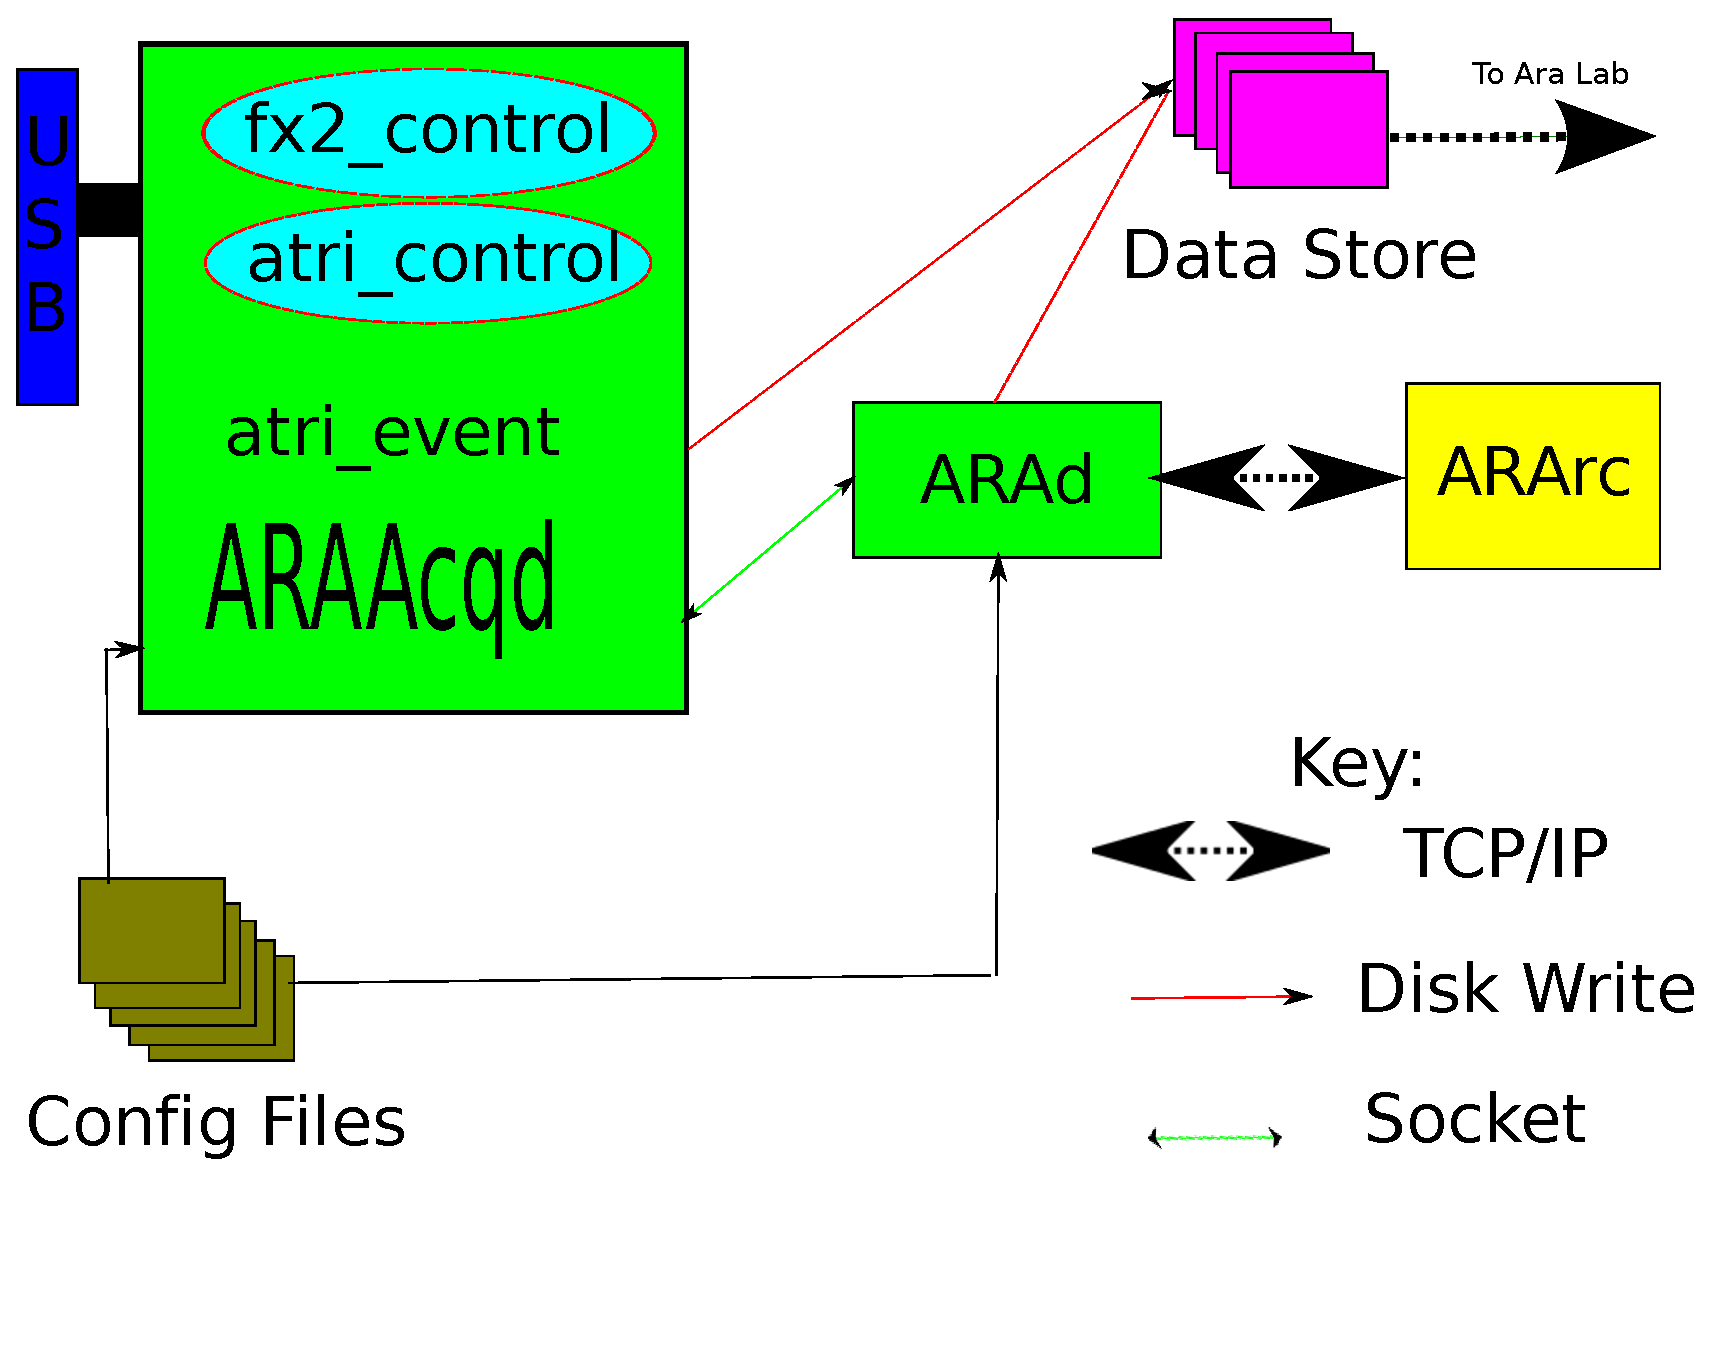
\includegraphics{araSoftDia.eps}}
  \caption{A schematic indicating the araSoft components and their methods of interaction. Currently the only piece of software which interfaces to the hardware is ARAAcqd which uses libusb to communicate with the ATRI board via the Cypress FX2 USB micro-controller. ARAAcqd provides two unix domain sockets (atri\_control and fx2\_control) which allow external programs to send a receive messages to/from the ATRI and FX2.}
  \label{fig:araSoftDia}  
\end{figure}


\subsection{Directory Tree}
All of the data is written into run directories, which contain event and housekeeping sub-directories. The location of the top directory is defined in the arad.config file
\begin{verbatim}
/data/run_000053/atriControl.log   -- debugging only
/data/run_000053/atriControlSent.log -- dbeugging only
/data/run_000053/atriEvent.log -- debugging only
/data/run_000053/event/ev_1314698257/ev_1314698257.168515.run000053.dat
/data/run_000053/eventHk/eventHk_1314698257/eventHk_1314698257.159373.run000053.dat
/data/run_000053/logs/runStart.log
/data/run_000053/peds/
/data/run_000053/sensorHk/sensorHk_1314698257/sensorHk_1314698257.039283.run000053.dat
\end{verbatim}

\section{ARA Software Processes}

\subsection{Program States}
The acquisition daemons (currently just ARAAcqd) are effectively state machines. The states are controlled by ARAd with the starting and stopping of runs. The program states are:
\begin{description}
\item[Idle] \hfill \\
  The program is idle and not actively taking event or housekeeping data. This is the default on program start.
\item[Preparing] \hfill \\
  The program is preparing and is initialising the hardware and opening output files, when completed the state automatically switches to prepared.
\item[Prepared] \hfill \\
  The program is ready to take data.
\item[Running] \hfill \\
  The program is actively taking data and writing to disk.
\item[Stopping] \hfill \\
  The program is stopping taking data and closing files, when completed the program will return to an idle state.
\item[Terminate] \hfill \\
  The program will stop and close.
\end{description}

\subsection{ARAAcqd}
The ARA Acquisition daemon (ARAAcqd) is the main workhorse program which is responsible for interfacing with the ATRI board via the USB micro-controller. This is a multithreaded program with five threads:

\begin{description}
  \item[Main thread] \hfill \\
    In addition to various setup functions (reading config files, starting the other threads, etc.) the main thread contains the event loop. In the event loop when the program is in the running state (see above) events are read out from the event endpoint and written to disk.
  \item[Housekeeping thread] \hfill \\
    The housekeeping thread contains an 'event' loop which in the running state (see above) reads out both the event and sensor housekeeping at the rate specified by the config file.
  \item[Run control thread] \hfill \\
    The run control thread opens a unix domain socket (acqd\_rc) and listens for instructions from the ARAd  daemon. Runs are started and stopped by ARAd sending appropriate control messages over this socket.
  \item[ATRI control socket thread] \hfill \\
    The ATRI control socket thread creates the atri\_control (and fx2\_control sockets) and  listens for atri control (fx2 control) packets which are sent to this thread. All packets sent to the atri\_packet\_controller are sent via this socket, including those sent from the other ARAAcqd threads. When a new packet is received it is assigned a packet number and placed in the packet queue for sending via the USB. FX2 control packets are all vendor requests~\cite{ref:fx2Note} and are sent as soon as they are received.
  \item[FX2 control thread] \hfill \\
    The FX2 control thread is responsible for actually reading from and writing to the control end point on the FX2. Packets are read from the packet queue and responses (which contain the packet number) are returned to the appropriate socket.
\end{description}

\subsubsection{Config File -- ARAAcqd.config}
There are several configuration variables defined in the ARAAcqd.config file. The current state of the ARAAcqd.config is:
\begin{verbatim}
//The ARAACqd config file
<log>
printToScreen#1=6;   //Controls the verbosity to screen
logLevel#I1=0; //Controls the verbosity to disk
atriControlLog#I1=0; //Enables the atriControl debug log
atriEventLog#I1=0; //Enables the atriEvent debug log
</log>

<acq>
doAtriInitialisation#I1=1; //Do the ATRI initialisation in the prepare phase
standAlone#I1=1; // Deprecated
numEvents#I1=100; // Deprecated
enableHkRead#I1=1; //Deprecated
eventHkReadRateHz#F1=2; //Readout rate of event housekeeping
sensorHkReadPeriod#I1=10; //Readout period (seconds) of sensor housekeeping
pedestalMode#I1=0; // Implemented
pedestalSamples#I1=10; // Number of events per block per pedestal run
pedestalDebugMode#I1=0; //Write out pedestal events
</acq>

<thresholds>
thresholdScan#I1=0;  //Perform a threshold scan
thresholdScanStep#I1=100; ///Threshold scan step size
thresholdScanPoints#I1=400; ///Number of threshold scan points
thresholdScanStartPoint#I1=0; ///Start value for the scan
setThreshold#I1=1; //Enable threshold setting
useGlobalThreshold#I1=0; //Enable a global threshold for all 16 DAC values
globalThreshold#1=20000; // The global threshold if enables
thresholdValues#I16=0,0,0,0,0,0,0,0,0,0,0,0,30000,30000,30000,30000; // The individual thresholds
setSurfaceThreshold#I1=0; // Actually set the surface thresholds?
surfaceBoardStack#I1=1; ///Which stack has a surface board 0-3 counting
surfaceThresholdValues#I4=1000,1000,1000,1000;
</thresholds>

<trigger>
numSoftTriggerBlocks#1=2; ///Number of software trigger blocks... must be even
enableSelfTrigger#I1=1; //Enable RF triggers
enableSoftTrigger#I1=1; //Enable timed software triggers
enableRandTrigger#I1=1; //Not yet implemented
softTriggerRateHz#F1=1.2; //Software trigger rate in Hz
randTriggerRateHz#F1=1.5; //Not yet implemented
</trigger>

<servo>
initialVadj#I4=17771,17771,17771,17771; ///< Initial Vadj
initialVdly#I4=43650,43650,54686,51114; ///< Initial Vdly
enableVdlyServo#I1=0; ///< Vdly servo for the wilkinson	
wilkinsonGoal#I1=125; ///< Goal target for the wilkinson		     
enableAntServo#I1=0; ///<Enables the antenna (L1) servo
scalerGoalValues#I16=0,0,0,0,0,0,0,0,500,500,500,500,0,0,0,0; ///< The 16 goal values for the ant servo
scalerPGain#F1=0.05; ///< Gain for the proportional part of the servo
scalerIGain#F1=0.01; ///< Gain for the integral part of the servo
scalerDGain#F1=0.00; ///< Gain for the differential part of the servo
scalerIMax#F1=100000; ///< Maximum integral value
scalerIMin#F1=-100000; ///< Minimum integral value
enableSurfaceServo#I1=0; ///Not yet implemented
surfaceGoalValues#I4=500,500,500,500; ///Not yet implemented			
enableRateServo#I1=1;  // Not yet implemented
servoCalcPeriodS#F1=1;  //Not yet implemented
servoCalcDelayS#F1=10;  //Not yet implemented
rateGoalHz#F1=5;  //Not yet implemented
ratePGain#F1=0.5; //Not yet implemented
rateIGain#F1=0.01; //Not yet implemented
rateDGain#F1=0.00; //Not yet implemented
rateIMax#F1=100; //Not yet implemented
rateIMin#F1=-100; //Not yet implemented 
</servo>
\end{verbatim}
The majority of the config options are either not yet enabled or are trivial switches or rate. A few of the more complicated options are described below:
\begin{description}
  \item[doAtriInitialisation] \hfill \\
    When this is set to 1, in the prepare phase a number of initialisation steps are carried out. This has the same effect has running clockset\_real.sh, doAtriInitialisation, atriSetVdly, atriSetVadj and enabling the IRS and wilkinson.
  \item[printToScreen and logLevel] \hfill \\
    These values control the verbosity printed to screen or log. Only messages with a higher priority (lower value) are printed/logged. The message priorities are
    \begin{enumerate}
      \setcounter{enumi}{-1}
    \item Emergency
    \item Alert
    \item Critical
    \item Error
    \item Warning
    \item Notice
    \item Info
    \item Debug
    \end{enumerate}
\item[thresholdScan] \hfill \\
  When this is enabled a threshold scan is performed and at the end ARAAcqd goes to idle. The threshold scan takes {\it thresholdScanPoints} starting at {\it thresholdScanStartPoint} spaced by {\it thresholdScanStep} DAC values.
\item[pedestalMode] \hfill \\
  When this is enabled a pedestal run is taking attempting to collect {\it pedestalSamples} events for each block
\item[initialVadj] \hfill \\
  This controls the IRS sampling rate within a block. At some point this needs to be servo'd to reliable obtain 3.2GSa/s. There is one number per DDA.
\item[initialVdly] \hfill \\
  This controls the slope of the Wilkinson ramp, it is less critical than Vadj and the servo mechanism is currently broken as the firmware gets stuck and reports the same number. There is one number per DDA.
\item[enableAntServo] \hfill \\
  This is the the single antenna threshold servo.
\item[scalerPGain,scalerIGain,scalerDGain,scalerIMin,scalerIMax] \hfill \\
  These are the parameters that should be tuned to produce an optimal servo.
\end{description}

\subsection{ARAd}
ARAd is the main control program on the station. The principle responsibilities of ARAd are periodically starting and stoppong runs and monitoring the health of the station. In addition ARAd interfaces with the global or local run control programs to allow user control of the data taking on the station.

\subsubsection{Config File -- arad.config}
The arad.config file contains configurable parameters for the ARAd daemon and defines the output data directories. The one parameter of interest in this config file is {\it restartRunsEvery} which sets the maximum run length in seconds. After this amount of time the run is restarted.
\begin{verbatim}
<output>
topDataDir#S=/data; //The data directory
linkDir#S=/data/link; //Link directory for transferring files 
linkForXfer#I1=1; //Actually make links for transferring files
filesPerDir#I1=100; //Files before need a new subdirectory
eventsPerFile#I1=100; //Events per file
hkPerFile#1=1000; // Hk objects per file
compressionLevel#I1=5; //zlib compression level
</output>

<log>
printToScreen#I1=8; //arad debugging level
logLevel#I1=0; ///arad logging level
</log>

<runControl>
startRunOnStart#I1=0;  ///< If set to 1 then ARAd will try and restart runs when it starts up
restartRunsEvery#I1=600; ///< If set to 0 will do nothing otherwise will restart runs every N seconds
</runControl>
\end{verbatim}


\section{Compiling}
In order to compile and run the software a number environmental variables are needed. An example setup script is included below:
\begin{verbatim}
#!/bin/bash
export ARA_DAQ_DIR=/home/ara/araSoft/trunk
export ARA_CONFIG_DIR=/home/ara/araSoft/trunk/config 
export LD_LIBRARY_PATH=${LD_LIBRARY_PATH}:${ARA_DAQ_DIR}/lib/
export DYLD_LIBRARY_PATH=${DYLD_LIBRARY_PATH}:${ARA_DAQ_DIR}/lib/
export PATH=${PATH}:${ARA_DAQ_DIR}/bin      
\end{verbatim}

\section{Running}

\subsection{Firmware}
The first step involved with running the program is to load the firmware onto both the FX2 micro-controller and the FPGA. Example scripts for this are on the araOhio machine. A suitable startup sequence would be:
\begin{verbatim}
sudo ~/fx2init_v1.0.sh 
FPGAPROG="/home/ara/repositories/ara/firmware/FX2/branches/v1.0/usbTools/FpgaProg/FpgaProg"
$FPGAPROG ~/atri_v6_6.bin 
sudo ~/fx2init.sh
\end{verbatim}

\subsection{Software}
Assuming that ARA\_DAQ\_DIR and ARA\_CONFIG\_DIR are defined the software can be run via scripts/startAraSoft.sh:
\begin{verbatim}
#!/bin/bash

cd /home/ara/araSoft/trunk
source setupAraDaqTesting.sh


nohup ARAd > arad.log 2>&1 &
nohup ARAAcqd > acqd.log 2>&1 &
nohup ./scripts/simpleDataPush.bash >datacopy.log 2>&1 &
\end{verbatim}

The run state can be controlled using startNewRun (to start a new run) and stopRun (to stop a run). The run log messages will be saved.

\subsubsection{Testing Software}
There are a number of useful programs in programs/testing, many of these have had the functionality recreated inside ARAAcqd. All of these programs requite ARAAcqd to be started (but it can be in idle mode) as they utilise the atri\_control and/or fx2\_control sockets provided by ARAAcqd. For debugging these programs are still useful, in particular:
\begin{description}
\item[atriGetDaughters] \hfill \\
Displays the status of the attached daughter boards.
\item[sendFx2ControlPacket] \hfill \\
Sends vendor command packets to the FX2, see \cite{ref:fx2Note} for more details.
\item[sendAtriControlPacket] \hfill \\
Sends packets to the atri\_packet\_controller, see \cite{ref:atriPacket} for more details.
\end{description}

\section{Output}
The current data structures are defined in araOneStructures.h. At present the simpleDataPush.bash script copies completed files from the SBC to the anitarf computer.


\begin{thebibliography}{0}
\bibitem{ref:atriDoc} P.~Allison, ``ATRI rev. B information'', ARA-DocDB-210, (2011)
\bibitem{ref:fx2Note} J.~Davies, ``EZUSB FX2LP Firmware For ATRI Board v1.0'', ARA-DocDB-288 (2011)
\bibitem{ref:atriPacket} P.~Allison, ``ATRI packet interface description'', ARA-DocDB-267, (2011)

\end{thebibliography}


 
\end{document}

